\documentclass[a4paper,11pt]{article}
\usepackage{a4wide}
\usepackage[english]{babel}
\usepackage{url}
\usepackage[latin1]{inputenc}
%\usepackage[small,bf,hang]{caption2}
\usepackage{xspace}
\usepackage{graphicx}
\usepackage{listings}
\usepackage{color}  
\usepackage[toc,page]{appendix}
\usepackage{subcaption}
\usepackage{pdflscape}
\usepackage{fixltx2e}
\usepackage{titlesec}

\newcommand{\HRule}{\rule{\linewidth}{0.5mm}}
\definecolor{mygreen}{rgb}{0,0.6,0}
\definecolor{mygray}{rgb}{0.5,0.5,0.5}
\definecolor{mymauve}{rgb}{0.8,0.4,0.2}
\definecolor{dkgreen}{rgb}{0,.6,0}
\definecolor{dkblue}{rgb}{0,0,.6}
\definecolor{dkyellow}{cmyk}{0,0,.8,.3}
\definecolor{gray}{gray}{0.6}

\lstset{
  backgroundcolor=\color{white},   % choose the background color; you must add \usepackage{color} or \usepackage{xcolor}
  basicstyle=\footnotesize,        % the size of the fonts that are used for the code
  breakatwhitespace=false,         % sets if automatic breaks should only happen at whitespace
  breaklines=true,                 % sets automatic line breaking
  captionpos=b,                    % sets the caption-position to bottom
  commentstyle=\color{mygreen},    % comment style
  deletekeywords={...},            % if you want to delete keywords from the given language
  escapeinside={\%*}{*)},          % if you want to add LaTeX within your code
  extendedchars=true,              % lets you use non-ASCII characters; for 8-bits encodings only, does not work with UTF-8
  frame=single,                    % adds a frame around the code
  keepspaces=true,                 % keeps spaces in text, useful for keeping indentation of code (possibly needs columns=flexible)
  keywordstyle=\color{blue},       % keyword style
  language=C++,                 % the language of the code
  morekeywords={*,...},            % if you want to add more keywords to the set
  numbers=none,                    % where to put the line-numbers; possible values are (none, left, right)
  numbersep=5pt,                   % how far the line-numbers are from the code
  numberstyle=\tiny\color{mygray}, % the style that is used for the line-numbers
  rulecolor=\color{black},         % if not set, the frame-color may be changed on line-breaks within not-black text (e.g. comments (green here))
  showspaces=false,                % show spaces everywhere adding particular underscores; it overrides 'showstringspaces'
  showstringspaces=false,          % underline spaces within strings only
  showtabs=false,                  % show tabs within strings adding particular underscores
  stepnumber=2,                    % the step between two line-numbers. If it's 1, each line will be numbered
  stringstyle=\color{mymauve},     % string literal style
  tabsize=2,                       % sets default tabsize to 2 spaces
  title=\lstname                   % show the filename of files included with \lstinputlisting; also try caption instead of title
}

\titlespacing{\section}{0pt}{\parskip}{-\parskip}
\titlespacing{\subsection}{0pt}{\parskip}{-\parskip}
%\titlespacing{\subsubsection}{0pt}{\parskip}{-\parskip}

\setlength{\parindent}{0cm}             % Inspringen van eerste lijn van paragrafen is niet gewenst.
\graphicspath{{figs/}}               % De plaars waar latex zijn figuren gaat halen.
\newcommand{\npar}{\par \vspace{2.3ex plus 0.3ex minus 0.3ex}}

\graphicspath{{figs/}}               % De plaars waar latex zijn figuren gaat halen.
% Nieuw commando om figuren in te voegen. Gebruik:
% \mijnfiguur[H]{width=5cm}{bestandsnaam}{Het bijschrift bij deze figuur}
\newcommand{\mijnfiguur}[4][!ht]{            % Het eerste argument is standaar `ht'. op H zetten voor HIER EN NERGENS ANDERS
    \begin{figure}[#1]                      % Beginnen van de figure omgeving
        \begin{center}                      % Beginnen van de center omgeving
            \includegraphics[#2]{#3}        % Het eigenlijk invoegen van de figuur (2: opties, 3: bestandsnaam)
            \caption{#4\label{#3}}          % Het bijschrift (argument 4) en het label (argument 3)
        \end{center}
    \end{figure}
}



\begin{document}
\begin{titlepage}
\pagenumbering{gobble}
\begin{center}

% Upper part of the page. The '~' is needed because \\
% only works if a paragraph has started.

\includegraphics[width=0.4\textwidth]{./logo}~\\[1cm]

% Title
\HRule \\[0.4cm]
\huge \textbf{Design of Multimedia Applications}
\HRule \\[0.4cm]
{ \huge \bfseries Report 2: Shot Detection \\[0.4cm] }
\HRule \\[0.4cm]

% Author and supervisor
\begin{minipage}{0.4\textwidth}
\begin{flushleft} \large
\emph{By:}\\
Andrea \textsc{Accogli}\\
Michiel \textsc{Creve}\\
Andreas \textsc{De Lille}\\
\end{flushleft}
\end{minipage}

\vfill

% Bottom of the page
{\large \today}

\end{center}
\end{titlepage}

\tableofcontents

\newpage
\pagenumbering{arabic}
\setcounter{page}{1}

\section[Pseudo-code and explanatory notes for the video shot detection method implemented
in Exercise 5.]{}\label{Q1}
The implemented method for exercise 5 is the Twin Comparison method\footnote{Based on 'Dissolve Detection Based On Twin-Comparison With Curve Fitting' by Yu et al.}. This method is based on the differences between the local histograms of subsequent frames. If the difference exceeds an upper threshold, this is seen as a hard cut. When the difference does not exceed the upper threshold, but exceeds a lower threshold, this frame is seen as the start of a possible soft cut. From then on, the differences of the next frames will be cumulatively summed. If this sum exceeds the higher threshold before a single frame-to-frame difference is lower than the lower threshold, a soft cut is detected.
\vspace{1em}
\begin{lstlisting}[frame=single]
bool DetectShot(double SampleTime, IntPtr pBuffer, int BufferLen){
	
	previous_histograms = current_histograms //save prev calculations
	List<int[]> current_histograms = new List<int[]>() //space for current
	
	for(every block){
        int[] local_histogram = new int[number of Bins * 3] //*3 for R, G and B
        
        for(every pixel in the block)
            // Increment histogram bin relative to R, G, B pixel value
            local histogram[corresponding red/green/blue bin]++;
        current_histograms.Add(local_histogram)
	}
	
	// Calculate difference between 2 histograms
	for(all histograms)
	    for(every bin in histogram)
	        difference = absolute value(previous bin value - current bin value)   

    Add difference to list of all differences of entire video
}
// If all frames played (all differences calculated), process data:
List<int> processData(){
    Calculate mean of all differences
    Calculate standard deviation of all differences
    
    // Start detecting cuts based on Twin Comparison
    List<int> listOfShots = new List<int>()
    higher threshold = alfa * mean + beta * stdev
    lower threshold = gamma * mean + delta * stdev
    for(all differences){
        differenceSum = 0;
        if(difference > higher threshold){
            add current framenumber to lisOfShots
        }else if(difference > lower threshold){
            int transitionLength = 0
            while(!last frame && difference > lower threshold && difference < higher threshold){
                differenceSum += difference
                increment framenumber (select next difference) 
                increment transitionLength
            }
            
            if(difference > higher threshold && last cut not within 10 frames)
                add current framenumber to lisOfShots // Hard cut detected
            else if(differenceSum > higher threshold && transitionlength >= 10){
                add current framenumber to listOfShots // Soft cut detected
        }
    }
    return listOfShots
}
\end{lstlisting}
\\
\section[A table documenting the different parameters used, as well as explanatory notes
regarding the definition and the range of these different parameters. Also, add a
rationale for the different parameter settings used (this is, how did you restrict the
parameter settings to a meaningful subset?).]{}The parameters used in exercise 5 are depicted in Table \ref{tab:twinparameters} in Appendix \ref{app:q2}. The parameters can be divided in 2 categories: Local Histogram and Twin Comparison. For the Local Histogram parameters, the number of blocks determines in how many blocks the frame will be divided. The number of blocks equals the number of histograms computed in one frame. Its value should be a number of which the square root is an integer (1, 4, 9, 16, 25, ...). The number of bins determines how many color values will be grouped in one bin. When the number of bins is 32, the number of values grouped in one bin will be 8 (= 256/32). The effect of changing the parameters listed in Table \ref{tab:twinparameters} will be addressed in the next question. 

The Twin Comparison parameters define the lower and the higher threshold. The upper and lower parameters are computed as follows:
\begin{center}
$lower \: threshold = alpha\times mean + beta\times stdev$\\$
higher \: threshold = gamma\times mean + delta\times stdev$
\end{center}
As the formula states, these thresholds depend on the average difference between frames in the video, and their standard deviation. This makes the thresholds adaptive: less 'turbulent' sequences will have lower thresholds, because of their lower mean difference. Their is no real restriction on the parameters, but experiments show that the parameters given in Table \ref{tab:twinparameters} yield satisfiable results. The effects of changing the parameters are discussed in the next question. Note that even tough these parameters yield satisfying results, further optimization could not be performed. Since that would require a huge set of video sequences in order to make the optimization scientifically correct. \\
\section[A comparative discussion of the precision and recall values obtained for each video shot detection method, taking into account different parameter settings.]{}
The recall and precision of all different implement methods are depicted in Table \ref{tab:precisionrecall} in Appendix \ref{app:q3-1}. Overall, the Twin Comparison method seems to score the best on the Star Wars sequence. In this question, this method will be used as an example to show the difference when changing parameters.

Changing thresholds has an impact on the precision and recall values. By lowering the thresholds, more cuts will be detected, resulting in lower recall and higher precision. This is so because false posive detections will also be amongst the frames that weren't detected with a lower threshold. Table \ref{tab:precisionrecall} confirms this statement.
 
Graphs showing the results for the CSI sequence using the Twin Comparison method are added in Appendix \ref{app:entire} and \ref{app:zoom}. Figure \ref{fig:entire} shows the difference between subsequent frames for the entire video. The lower and higher threshold, ground truth and detected shots are also shown in the figure. In order to show the results more precise, Figure \ref{fig:zoom} zooms in on frames 0-800. One can notice that in these sequence all detected cuts are hard cuts, where the difference exceeds the higher threshold. Although the graph shows satisfiable results, there are still some faults in the detection.
 
The first mistake lies around frame 400, where the difference exceeds the lower threshold (but does not exceed the higher). These differences sum up to the higher threshold, resulting in a wrongly detected cut (= a false positive). The cause for this is a highly turbulent sequence of frames: a toilet being flushed. A print screen of this is shown in Figure \ref{fig:flush} in Appendix \ref{app:turbulent}.

The second noticeable mistake lies around frame 780. Here, two shots dissolve into each other, as shown in Figure \ref{fig:dissolve} in Appendix \ref{app:dissolve}. The dissolve stars around frame 750, which explains the increase in difference starting from that frame. The difference however does not exceed the lower threshold, which causes a false negative: the shot at frame 785 is not detected by the Twin Comparison. If the lower threshold would be lowered, the system will be able to detect this transition, but it will also include the detection of new false positives, probably somewhere around frames 90, 580 and 650.

Also, note that for some shots several high differences appear. An example of this is the hard cut at frame 111. Here, some other peak values appear after this frame. To filter these out, the system ignores all cuts within 10 frames of the previous cuts. The graph shows that this intervention filters out all these 'burst detections'.
\\
\section[A comparative discussion of the computational complexity of each video shot detection method, taking into account different parameter settings. Provide information about the PC configuration used in order to put the time measurements in context.]{}

\subsection{Configuration}
A detailed setup is found in Section \ref{q4:setup} of Appendix \ref{app:q4}. The used video sequence is, unless stated different, \emph{return\_jedi\_trailer\_cuts-only.avi}, that has a resolution of 352x176 pixels, a total of 1736 frames that run with a framespeed of 25 frames/second for 69 seconds.
\\
\subsection{Pixel method}
The shot detection has no parameters that influence the complexity or timing of the algorithm in any way and executes the star wars sequence with a delay of 6.93 ms/frame. 
\\
\subsection{Motion method}
The motion estimation has 2 parameters that both influence the timing, the size of a sub block and the search window. A larger sub block size results in less motion estimations, but each motion estimation takes longer since the difference is determined by calculating the absolute difference for each pixel inside the subblock. The search window also influences the execution time: a larger search window, means that more iterations of the logarithmic motion estimation are needed. Table \ref{execMotion} in Appendix \ref{app:q4} gives the processing times of the algorithm for different sub sizes and search window sizes. Generally speaking, one trend can be seen: a greater search window results in slower execution time while the influence of the subsize is negligable.
\\
\subsection{Global histogram}
The global histogram only has one parameter that influences the execution time: the bin count. A higher bin counts means that some additional processing is needed. Table \ref{execGlobal} in Appendix \ref{app:q4} shows the different execution times: it is clear that the binCount has very little or no influence on the execution time.
\\
\subsection{Local histogram}
The local histogram divides the frame in different regions and then executes the global histogram method on each region. It has 2 parameters that influence the execution times: the number of regions and the binCount. As shown in the global histogram method, the bin count has a negligible influence on the execution time. Thus only the difference in regions is considered and the binCount is set to 32 for all executions. The results  in Table \ref{execLocal} of Appendix \ref{app:q4} show that the influence of the region count on the execution time is also very little.
\\
\subsection{Twin Comparison}
The execution times of the Twin Comparison method are shown in Table \ref{twincomp} in Appendix \ref{app:q4}. These times show the same trend as the local histogram methods. This is normal, since the twin comparison method is an extension of the local histogram method.
\\
\section[A summarizing ROC curve for each video sequence, illustrating the effectiveness of the different techniques implemented (see slide 26 of the introductory lecture). Corresponding tables need to be provided as well, containing the optimal parameter settings and the resulting precision, recall, and F1 score (the harmonic mean of precision and recall).]{}

The tables are included in \ref{ROCTable1} and \ref{ROCTable2} of Appendix \ref{app:q5}. The curves are in Figure \ref{rocPixel}, Figure \ref{rocMotion}, Figure \ref{rocGlobalLocal} and Figure \ref{rocTwin} of Appendix \ref{app:q5}. The optimal values, precision, recall and F1 values can be found in Table \ref{ROCValues} in Appendix \ref{app:q5}. 

It can be concluded that these methods all scale differently, but one common trend is observed. A higher recall usually means that the precision is lower. This is explained as follows, a higher recall corresponds with higher thresholds. This means that not all shots are detected, but the probability that the detection really is a shot, is higher. The recall / precision is a trade-off that should be chosen with care. On one hand, one can either go for a trustworthy method, that does not detect all shots, with the benefit of having less false detections. On the other hand a sensitive method, that finds more shots at the cost of having some false detections is also possible.
\\
\section[A discussion of the differences between the video shot detection methods, and the influence of these differences on 1) the precision and recall values and 2) the computational complexity]{}

As shown in Figure \ref{grafiek} in Appendix \ref{app:q6}, the pixel method, while being very simple, achieves quite reasonable results when calibrated right. The second method is the motion method, whose results are better since it gets less confused by motion. However, the results are far from perfect. In an experimental attempt to optimize this method, an auto mode was implemented. This auto mode keeps track of the average of the difference between frames and reports a shot when the current difference exceeds a multiple of the average. This method is among the best ones, but is slow due to the complex motion estimation. This problem is easily solved using a speedup, a speedup of 4 means that the motion algorithm only processes 1 in 4 blocks. These speedups are useful for high resolution sequences.

Next up are the histogram methods, where the local histogram scores a lot better than the global histogram, due to its ability to detect more fades and more difference in the frame (because it checks for local differences). For instance, if only the camera angle changes between shots, then the average color values will still be more or less the same, but the colors will appear at different places. The local method does detect this by checking averages per region instead of one global average. The added complexity for the local histogram method is thus justified with higher results.

The winner for the star wars method for precision and recall is the twin comparison, which has the highest precision (94\%) and recall (92\%), while also being the fastest method. This is no surprise, since the twin comparison is the most complex method. Given its score, the added complexity is certainly justified here. Even though the results are high, they are not perfect, this is because twin comparison does a bad job at detecting dissolves.
\\
\section[An answer, with explanation, to the following questions:]{}

\subsection[Can a clear winner be found among all different video shot detection methods and parameter settings?]{}
All methods have their up- and downsides. However, the Twin comparison is the winner for the simple reason that is capable of detecting fades. This method has a recall of 92\% and a precision of 94\%. This is not perfect, since twin comparison does not detect most dissolves. Note that the auto motion, even though it was not designed for the CSI sequence, still provides good results with 96\% recall and 90\% precision. However since the motion is very slow for high resolution frames, a speedup of 10 was used during the execution, this means that only 1 in 10 subblocks was processed.
\\
\subsection[For the clear winner found, or for the video shot detection method that you would use in practice:]{}
\subsubsection[How would you further improve this method in terms of precision?]{}
The problem here is that the thresholds are more or less fixed (they rely on the mean difference and standard deviation in the sequence), while each video and each shot has its own characteristics. Some shots contain a lot of motion, while others move more slowly, thus the accuracy and precision of a static threshold has an upper limit. In an experimental approach to solve this, the motion method was extended with an additional auto mode, that keeps an average of the difference of the frames. In order to avoid a second passing through the frames, the average is approximated in real time with following formula: $AvgDiff = AvgDiff * X + currDiff * Y$ with the requirement: $X+Y = 1$. A higher X means that the video is less sensitive for quick changes in the sequence.

This provided higher precision (78\% compared to 61\%), but a slightly lower recall (only 84\% instead of 90\%) for the motion estimation technique. This technique was not applied to the twin comparison, but it is expected to receive the same results, especially when multiple sequences are used.
\\
\subsubsection[How would you further improve this method in terms of processing speed?]{}
The easiest way to speedup the algorithms is to consider a small subset of the frame. The delivered source code applies this for the motion estimation. A speedup of 5 means that only 1 in 5 subblocks is processed. The results of high resolution video sequences, such as the CSI sequence were not or very little affected by this speedup. However the impact on low resolution sequences, e.g. the star wars sequence, was much more dramatically. The results also indicated that the auto mode responded better to the speedup of low resolution sequences, due to the dynamic character of the auto mode.

This could also be applied to the twin comparison method, where only a few sub blocks in each region are processed to speedup the execution. Even though the technique was not applied to the twin comparison method, similar results of the motion method are expected. Additionally executing the algorithm in parallel, could significantly speedup the execution, since it would use the full potential of the different cores that most laptops have.
\\
\subsection[What is the obvious shortcoming in practical scenarios, that the different video
shot detection methods have in common, and how would you deal with this?]{}
The first problem is the detection of fades in a sequence, the fades are not (always) detected by the simple algorithms. The Twin Comparison method provides a solution, but still has difficulties with the detection of dissolves. To detect these transitions, more complex algorithms are needed. 

Another problem was that some detection algorithms detect in bursts (a shot is detected multiple times). To solve this, detections within 10 frames of the previous shot are ignored.

To conclude, it is believed that even the most complex algorithms are not perfect, thus it would be advisable for the user to manually correct the detected shots in his video. The process would then be semi-supervised, first the user would upload the video and then a shot detection algorithms would be preformed. Once ready, the user can annotate and correct the shots. 
\\
\subsection[Given a video sequence produced by a wearable computing device like Google Glass (a/o), what issues does a method for video shot detection need to overcome?]{}
The shot detection can either happen online (in real time) or offline. Given the limitations of wearables, such as limited processing power and battery life, it would be advisable to run the shot detection in server farms where these limitations are neglected. One could consider the low resolution of the camera of wearables. Even though it is true that the resolution of video sequences produced by wearable computing devices usually is a bit lower than the average digital camera, but that is not the biggest problem. On the contrary, the lower resolution reduces the computing time of the shot detection. The downside might be that the results could be less accurate.

Another problem might be the limited color depth of the wearable's camera, which determines the amount of bits used to encode the color of a single pixel. Limited color depth will result in less distinguishable colors, which might cause problems for the shot detection: new colors in fades could have less difference and therefore the fade might not be detected. 

However, the greatest problem would be the instability of the camera, video sequences recorded with wearables are usually not very stable. The result of this is a 'motion pollution' that might confuse shot detection algorithms, e.g. the pixel algorithm would find a lot of difference between the pixels, caused by this motion.
\\
\subsection[Why is it important to add meta data to video content?]{}
The Internet contains vast amounts of video content, this content is more valueable if it can be found by a search. In order to make this vast amount of video content searcheable, tags and annotations are needed. Searching a video of e.g. a car is very hard without this meta data. The computer system has no clue as to what videos contain a car. Apart from searching, meta data are also used for organizing and categorizing the content.
\\
\subsection[Given the annotation and retrieval functionality of the application written, what are some of the (engineering/user) problems that you foresee when you would deploy this application in the real world?]{}
Scalability: to search a large collection of video clips you need storage for the content and annotations. The annotations themselves should be accessible without too much overhead. You would also need semantics to link different synonyms together, one might tag an object as a \emph{car} while someone else might call it an \emph{automobile}. It is quite obvious that, since these words are related, the result of a search operation for the tag \emph{car} should contain both the results for \emph{car} and \emph{automobile}.
\clearpage
\begin{appendices}

%\section{Q1}\label{app:q1}
%\clearpage

\section{Q2}\label{app:q2}
\begin{table}[h]
\centering
\caption{Overview of parameters used in exercise 5}
\label{tab:twinparameters}
\begin{tabular}{|c|clcc}
\cline{1-1} \cline{4-4}
\multicolumn{1}{|l|}{\textbf{Twin Comparison}} & \multicolumn{1}{l}{\textbf{}} & \multicolumn{1}{l|}{} & \multicolumn{1}{c|}{\textbf{Local Histogram}}           &                         \\ \cline{1-2} \cline{4-5} 
\textit{\textbf{Alfa}}                         & \multicolumn{1}{c|}{1.5}      & \multicolumn{1}{l|}{} & \multicolumn{1}{c|}{\textit{\textbf{Number of bins}}}   & \multicolumn{1}{c|}{32} \\ \cline{1-2} \cline{4-5} 
\textit{\textbf{Beta}}                         & \multicolumn{1}{c|}{0.0}      & \multicolumn{1}{l|}{} & \multicolumn{1}{c|}{\textit{\textbf{Number of blocks}}} & \multicolumn{1}{c|}{9}  \\ \cline{1-2} \cline{4-5} 
\textit{\textbf{Gamma}}                        & \multicolumn{1}{c|}{1.0}      &                       & \multicolumn{1}{l}{}                                    & \multicolumn{1}{l}{}    \\ \cline{1-2}
\textit{\textbf{Delta}}                        & \multicolumn{1}{c|}{2.0}      &                       & \multicolumn{1}{l}{}                                    & \multicolumn{1}{l}{}    \\ \cline{1-2}
\end{tabular}
\end{table}

\section{Q3}\label{app:q3}
\subsection{Recall and precision of the different implemented methods}\label{app:q3-1}
\begin{table}[h]
\centering
\caption{Recall and Precision of the different implemented methods}
\label{tab:precisionrecall}
\begin{tabular}{|l|l|l|l|}
\hline
\textbf{Method}  & \textbf{Sequence} & \textbf{Recall (\%)} & \textbf{Precision (\%)} \\ \hline
Pixel            & Star Wars       & 74                   & 75                      \\ \hline
Motion           & Star Wars       & 90                   & 61                      \\ \hline
Global Histogram & Star Wars       & 83                   & 62                      \\ \hline
Local Histogram  & Star Wars       & 82                   & 85                      \\ \hline
Twin Comparison  & Star Wars       & 82                   & 86                      \\ \hline
Twin Comparison  & CSI               & 92                   & 94                      \\ \hline
\end{tabular}
\end{table}

\clearpage
\subsection{Twin Comparison graph: entire video}
\label{app:entire}

\begin{figure}[!ht]
  \centering
  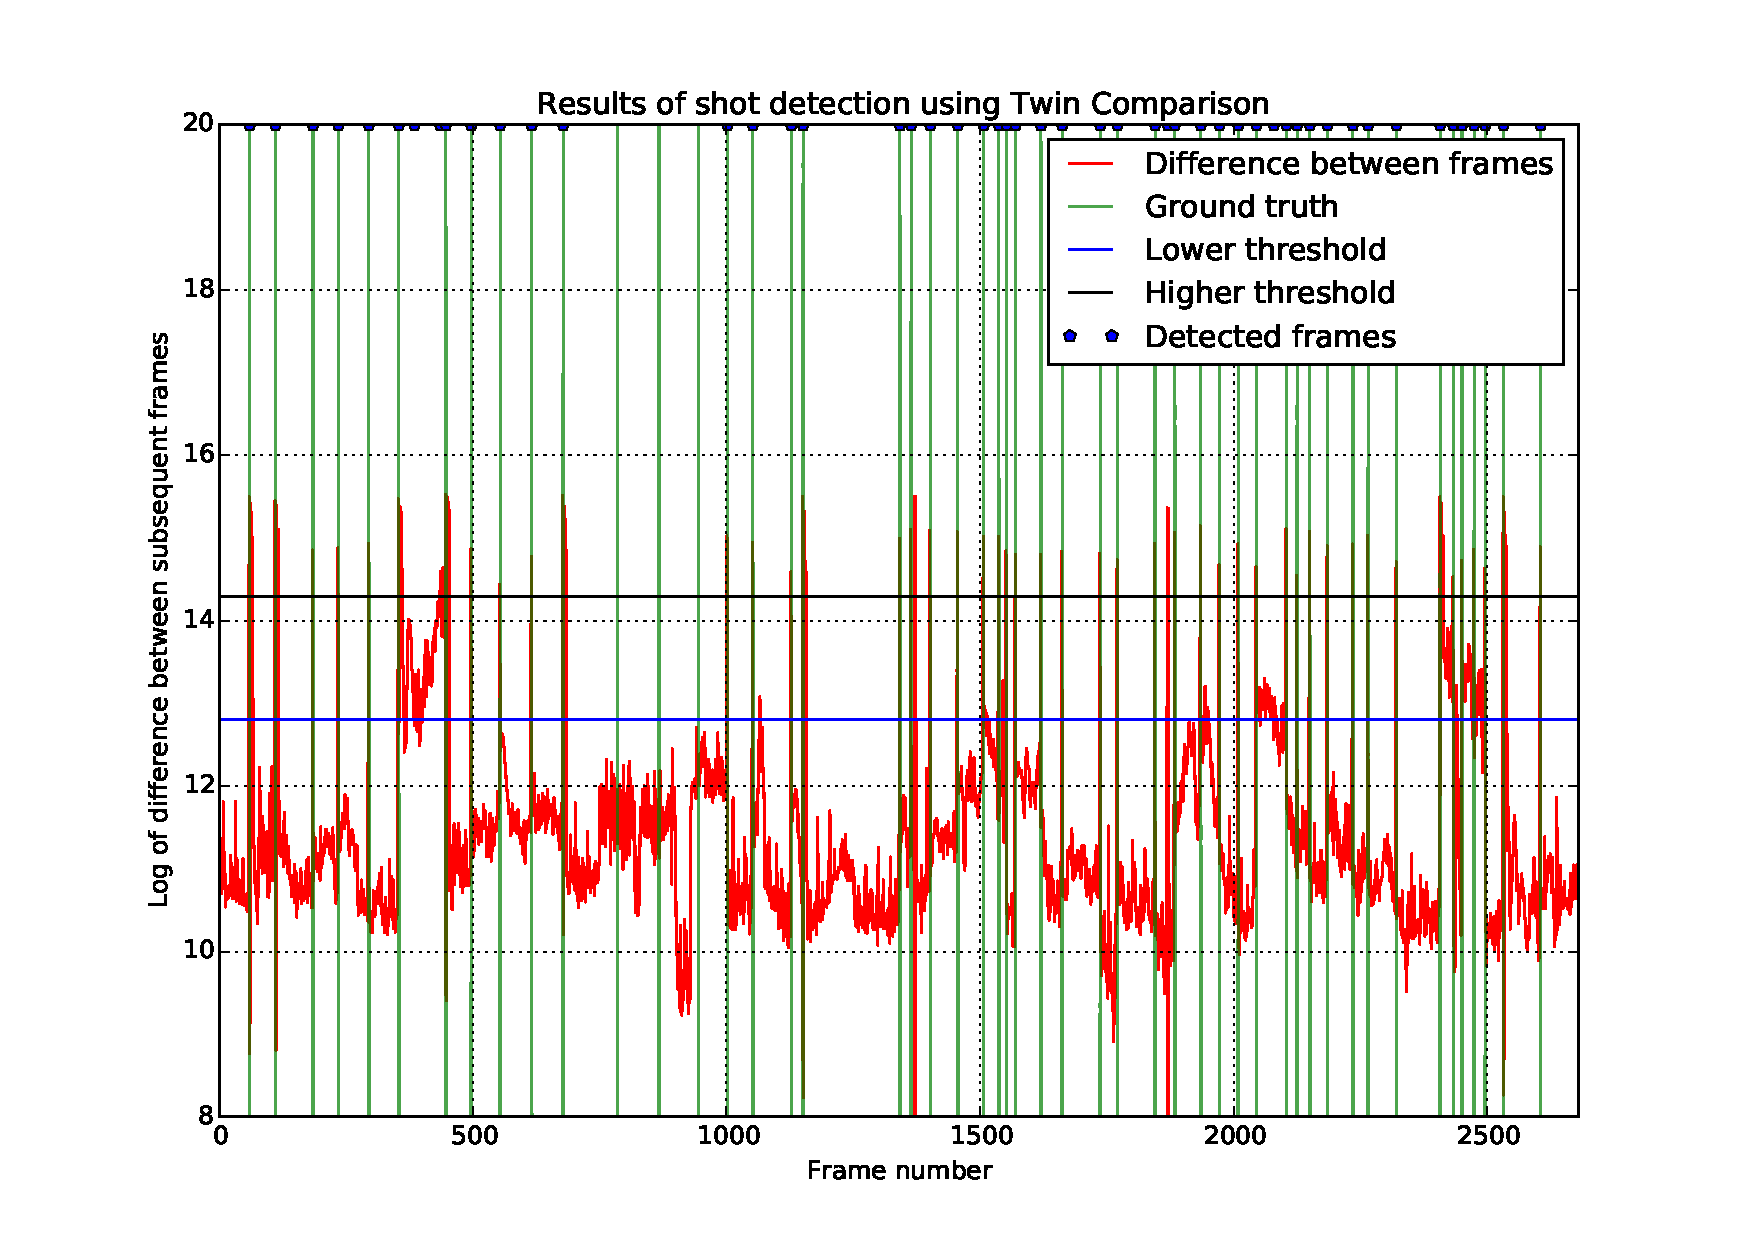
\includegraphics[page=1,angle=90,height=0.9\textheight,keepaspectratio]{figs/graph_entire_video}
  \caption{Results of Twin Comparison: entire video}
  \label{fig:entire}
\end{figure}

\newpage
\subsection{Twin Comparison graph: frame 0-800}
\label{app:zoom}

\begin{figure}[!ht]
  \centering
  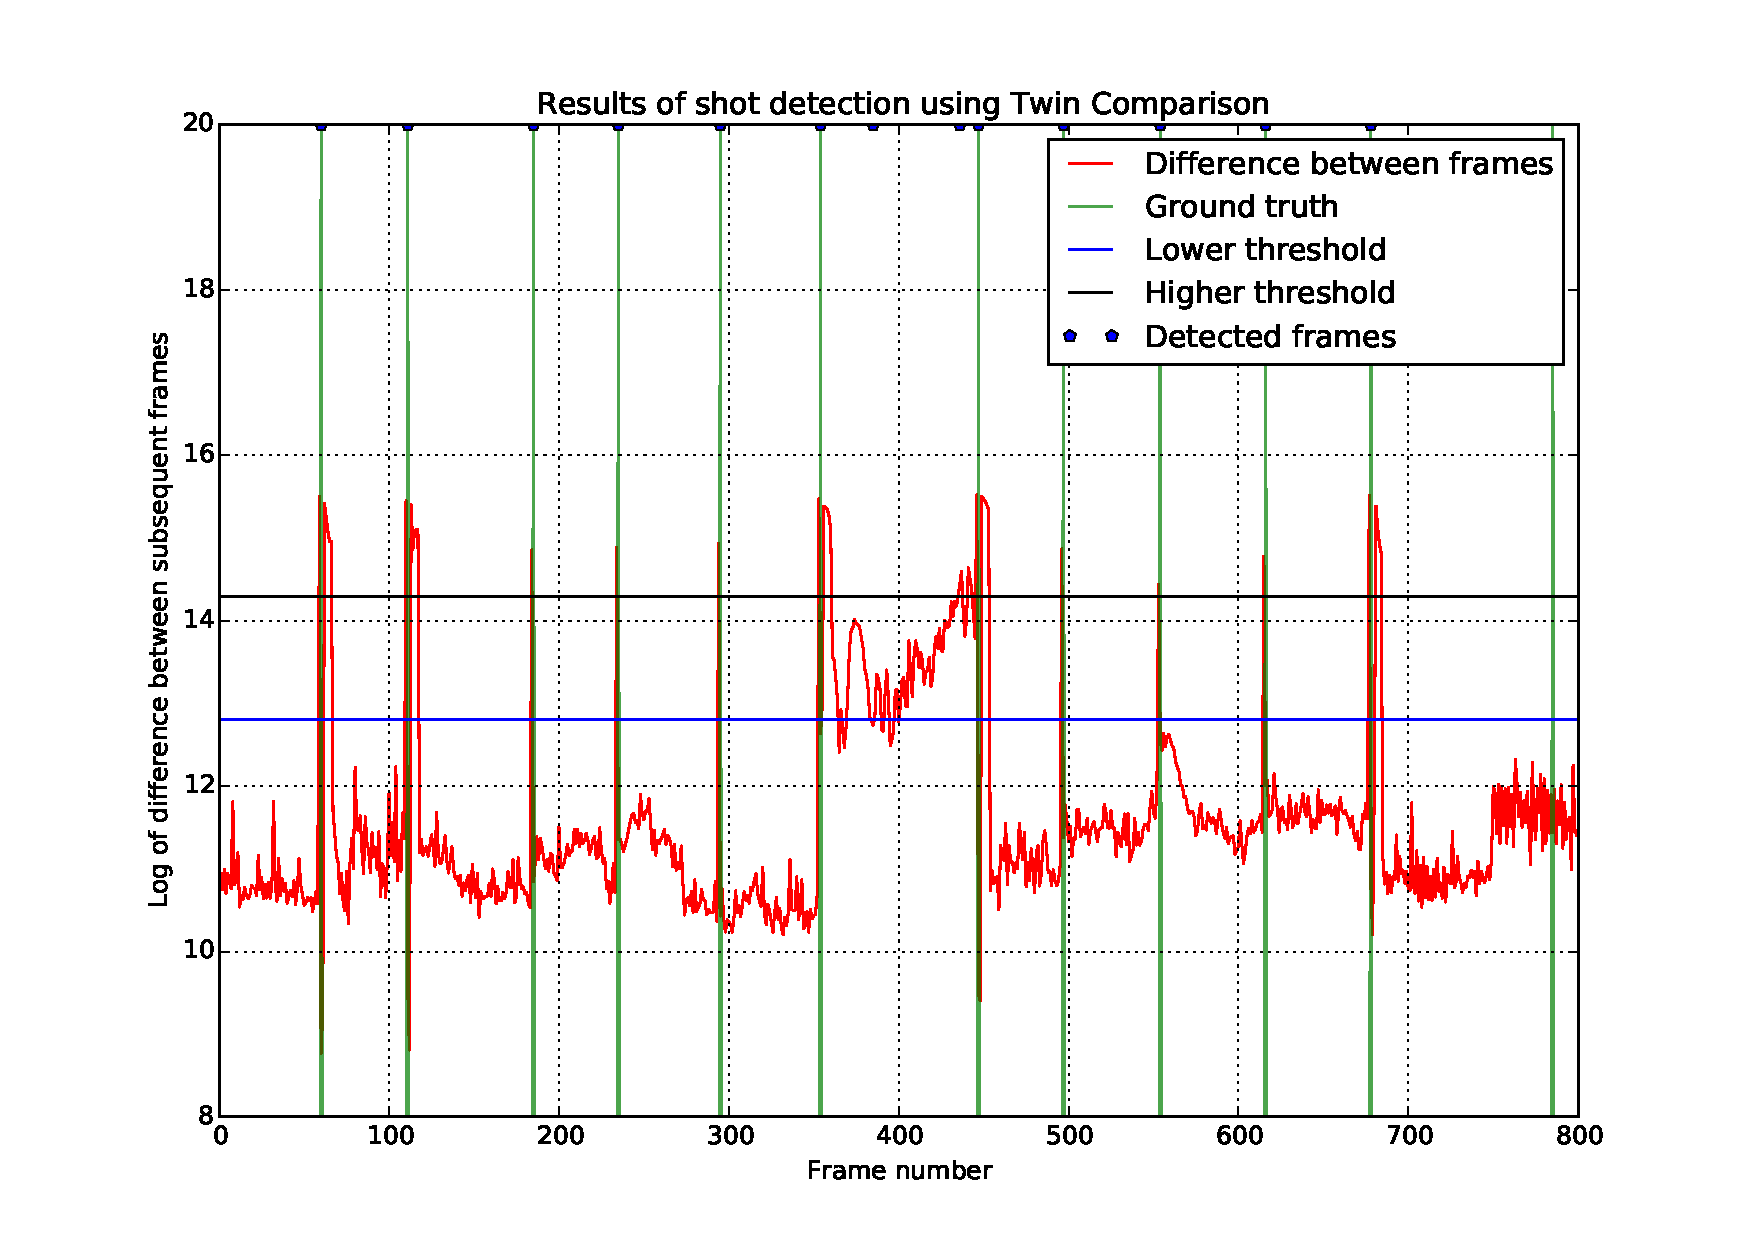
\includegraphics[page=1,angle=90,height=0.9\textheight,keepaspectratio]{figs/graph_zoom}
  \caption{Results of Twin Comparison: frame 0-800}
  \label{fig:zoom}
\end{figure}

\newpage

\subsection{Cause for false positives: Turbulent Sequences}
\label{app:turbulent}
\begin{figure}[ht]
  \centering
  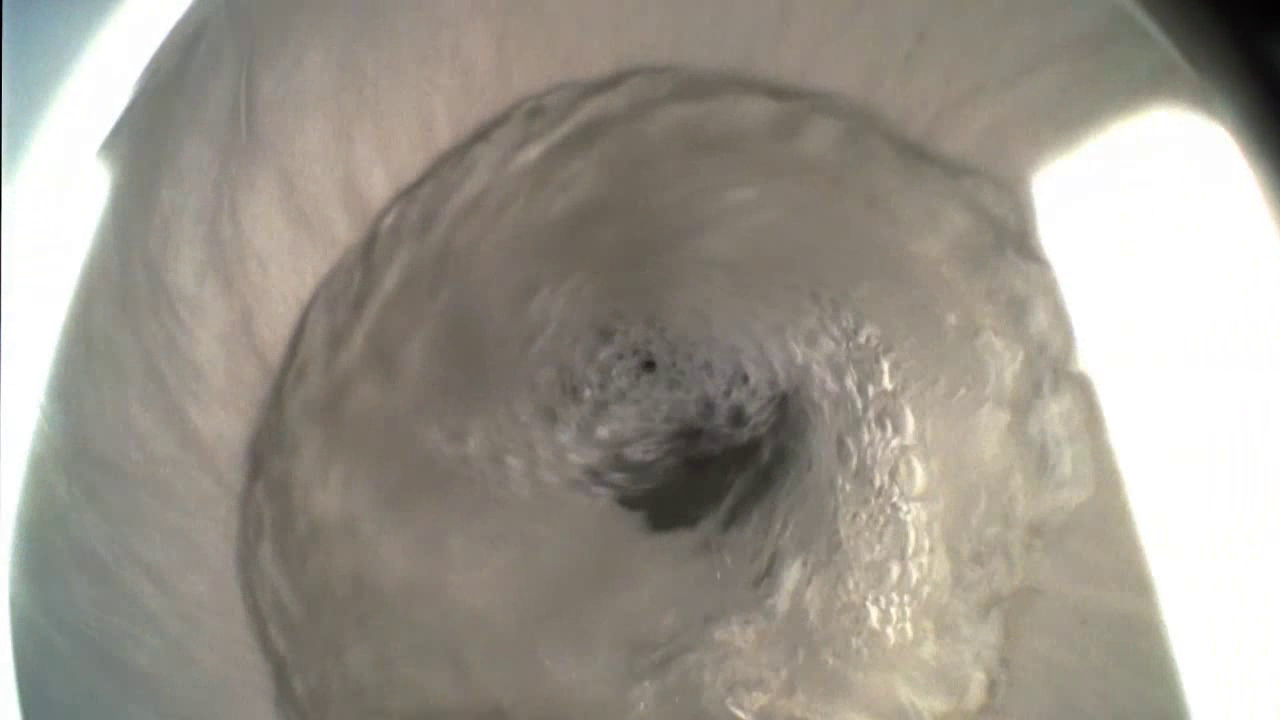
\includegraphics[width=.85\textwidth]{figs/turbulent}
  \caption{Turbulent sequences cause false positives}
  \label{fig:flush}
\end{figure}


\subsection{Cause for false negatives: Dissolves}
\label{app:dissolve}
\begin{figure}[ht]
  \centering
  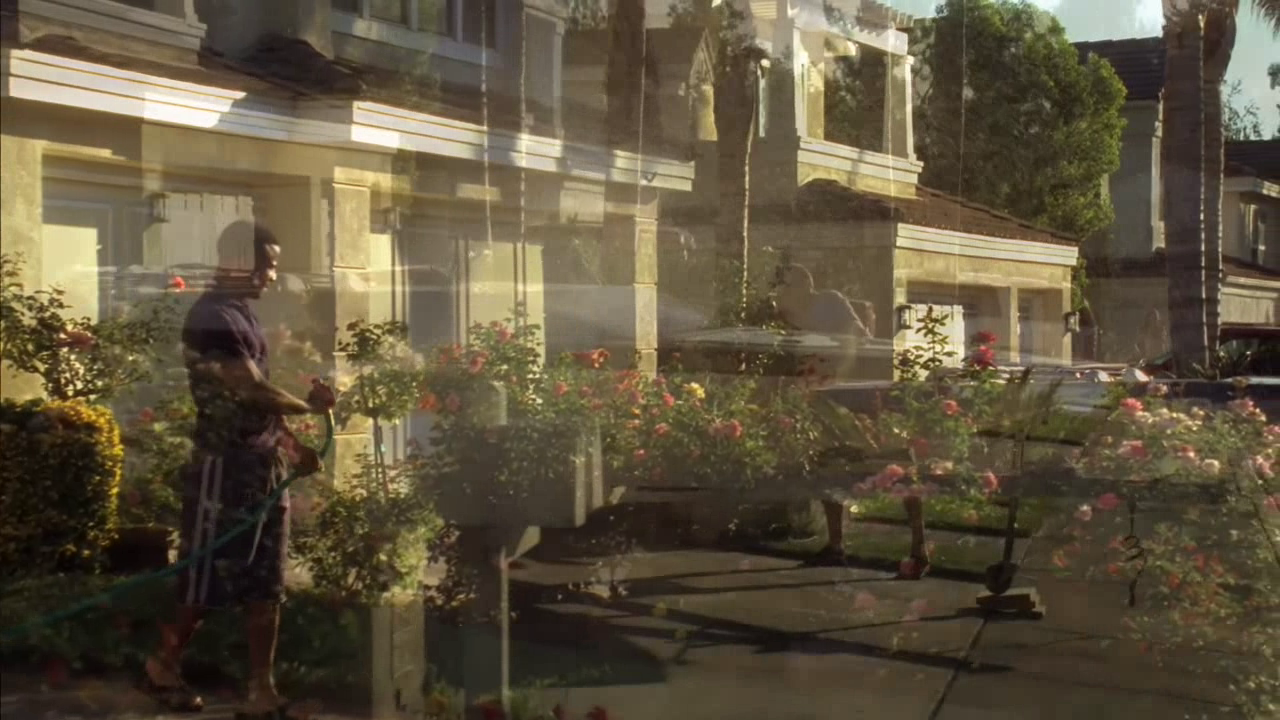
\includegraphics[width=.85\textwidth]{figs/dissolve}
  \caption{Dissolving transitions are hard to detect}
  \label{fig:dissolve}
\end{figure}

\newpage
\section{Q4}\label{app:q4}

\subsection{Setup}\label{q4:setup}
The used setup for all timings is: PC Configuration used for the measurements: 
\begin{enumerate}
\item Intel i5, 2 cores, 4 threads @2.5ghz 
\item 8GB dual-channel DDR3 @798Mhz RAM. 
\item GPU: Integrated Intel Hd graphics 4600 + NVIDIA GeForce GT 740M (2048MB dedicated RAM). 
\item The HD is a 700GB SATA-III 5400 RPM.
\end{enumerate}

\begin{table}[!ht]
\caption{Execution times (ms/frame) of different subsizes and search window sizes for the motion estimation.}
\label{execMotion}
\begin{tabular}{|l|l|l|l|l|l|l|}
\hline
\textbf{subSize (right)}\\ \textbf{searchWindow (below)}& \textbf{2} & \textbf{4} & \textbf{8} & \textbf{16} & \textbf{32} & \textbf{64} \\ \hline
\textbf{9}  & 49.36 & 41.33 & 46.78 & 42.26 & 42.63 & 47.64 \\ \hline
\textbf{11} & 48.60 & 40.33 & 44.05 & 42.05 & 42.31 & 40.08 \\ \hline
\textbf{15} & 51.07 & 43.10 & 44.30 & 43.23 & 40.51 & 39.36 \\ \hline
\textbf{19} & 87.80 & 85.20 & 80.47 & 82.22 & 77.30 & 80.21 \\ \hline
\end{tabular}
\end{table}

\begin{table}[!ht]
\caption{Execution times (ms/frame) of different bin counts for the global histogram method.}
\label{execGlobal}
\begin{tabular}{|l|l|l|l|l|l|l|l|l|l|l|}
\hline
\textbf{binCount}       & \textbf{25} & \textbf{50} & \textbf{75} & \textbf{100} & \textbf{125} & \textbf{150} & \textbf{175} & \textbf{200} & \textbf{225}  \\ \hline
\textbf{Execution time} & 2.36       & 2.62     & 2.38       & 2.62      & 2.83      & 2.37      & 2.32      & 2.32      & 2.35       \\ \hline
\end{tabular}
\end{table}

\begin{table}[!ht]
\caption{Execution times (ms/frame) of different region counts for the local histogram method.}
\label{execLocal}
\begin{tabular}{|l|l|l|l|l|l|l|l|l|l|l|}
\hline
\textbf{regionCount}    & \textbf{4} & \textbf{9} & \textbf{16} & \textbf{25} &\textbf{36}  & \textbf{49} & \textbf{64} & \textbf{81} \\ \hline
\textbf{Execution time} & 5.33    & 5.01     & 5.06     & 5.00     & 5.12     & 5.04     & 5.31     & 4.98     \\ \hline
\end{tabular}
\end{table}

\begin{table}[!ht]
\caption{Execution times (ms/frame) of different region counts for the Twin Comparison method.}
\label{twincomp}
\begin{tabular}{|l|l|l|l|l|l|l|l|l|l|l|}
\hline
\textbf{regionCount}    & \textbf{4} & \textbf{9} & \textbf{16} & \textbf{25} & \textbf{36} & \textbf{49} & \textbf{64} & \textbf{81} \\ \hline
\textbf{Execution time} & 5.20   & 5.22    & 5.04     & 5.22     & 5.17     & 5.34     & 5.43  & 5.75    \\ \hline
\end{tabular}
\end{table}

\section{Q5}\label{app:q5}
\subsection{Tables}

\begin{landscape}
\begin{table}[!ht]
\centering
\caption{ROC table part 1}
\label{ROCTable1}
\begin{tabular}{|l|l|l|l|l|l|l|}
\hline
\textbf{recall} & \textbf{pixelDistance} & \textbf{pixelFraction} & \textbf{motionDistance} & \textbf{motionFraction} & \textbf{globalFraction} & \textbf{localFraction} \\ \hline
\textbf{9}      &                        & 98                     & 90                      & 90                      &                         &                        \\ \hline
\textbf{23}     &                        & 98                     &                         &                         & 97                      &                        \\ \hline
\textbf{36}     & 92                     &                        &                         &                         &                         & 90                     \\ \hline
\textbf{50}     &                        &                        &                         &                         & 86                      &                        \\ \hline
\textbf{52}     &                        & 88                     &                         &                         &                         & 88                     \\ \hline
\textbf{57}     & 86                     &                        &                         &                         &                         &                        \\ \hline
\textbf{71}     & 71                     &                        &                         &                         &                         &                        \\ \hline
\textbf{76}     &                        &                        &                         &                         & 84                      &                        \\ \hline
\textbf{77}     &                        &                        &                         & 84                      &                         &                        \\ \hline
\textbf{78}     &                        &                        & 80                      &                         &                         &                        \\ \hline
\textbf{82}     & 29                     &                        &                         &                         &                         & 86                     \\ \hline
\textbf{83}     & 20                     & 51                     &                         &                         &                         &                        \\ \hline
\textbf{84}     &                        &                        & 76                      &                         & 63                      &                        \\ \hline
\textbf{88}     &                        &                        &                         & 43                      &                         &                        \\ \hline
\textbf{89}     &                        &                        &                         &                         &                         & 78                     \\ \hline
\textbf{90}     &                        &                        & 61                      &                         &                         &                        \\ \hline
\textbf{91}     &                        &                        & 55                      &                         & 41                      &                        \\ \hline
\textbf{93}     &                        &                        &                         &                         &                         & 51                     \\ \hline
\textbf{100}    &                        & 2                      &                         & 17                      & 2                       & 2                      \\ \hline
\end{tabular}
\end{table}
\end{landscape}


\begin{landscape}
\begin{table}[!ht]
\centering
\caption{ROC table part 2}
\label{ROCTable2}
\begin{tabular}{|l|l|l|l|l|}
\hline
\textbf{recall} & \textbf{TwinAlfa} & \textbf{TwinBeta} & \textbf{TwinGamma} & \textbf{TwinDelta} \\ \hline
\textbf{9}      &                   & 90                &                    &                    \\ \hline
\textbf{36}     &                   &                   &                    & 84                 \\ \hline
\textbf{43}     & 87                &                   &                    & 82                 \\ \hline
\textbf{56}     &                   & 87                &                    &                    \\ \hline
\textbf{58}     &                   &                   &                    & 78                 \\ \hline
\textbf{67}     &                   &                   &                    & 78                 \\ \hline
\textbf{72}     &                   &                   &                    & 76                 \\ \hline
\textbf{73}     & 86                &                   &                    &                    \\ \hline
\textbf{74}     &                   &                   &                    &                    \\ \hline
\textbf{75}     & 84                &                   & 82                 & 73                 \\ \hline
\textbf{76}     &                   & 83                & 84                 & 63                 \\ \hline
\textbf{77}     &                   &                   & 73                 &                    \\ \hline
\textbf{78}     &                   &                   & 73                 &                    \\ \hline
\textbf{82}     &                   & 67                &                    &                    \\ \hline
\textbf{84}     & 57                &                   &                    &                    \\ \hline
\textbf{87}     &                   &                   &                    & 37                 \\ \hline
\textbf{91}     & 22                &                   &                    &                    \\ \hline
\textbf{100}    &                   & 2                 &                    &                    \\ \hline
\end{tabular}
\end{table}
\end{landscape}
\clearpage

\subsection{ROC curves}
\subsubsection{Pixel}
\mijnfiguur{width=\textwidth}{rocPixel}{ROC curve for the pixel method (both distance and fraction variations)}
\subsubsection{Motion}
\mijnfiguur{width=\textwidth}{rocMotion}{ROC curve for the motion method (both distance and fraction variations)}
\clearpage
\subsubsection{Local and Global}
\mijnfiguur{width=0.9\textwidth}{rocGlobalLocal}{ROC curve for both the local and global histogram methods}
\subsubsection{Twin Comparison}
\mijnfiguur{width=0.9\textwidth}{rocTwin}{ROC curve for the twin comparison method (for alpha, beta, gamma and delta)}
\clearpage

\begin{landscape}
\begin{table}[h]
\caption{Precision, recall and F1 value for the different methods}
\label{ROCValues}
\begin{tabular}{|l|l|l|l|l|l|l|l|l|l|l|l|l|l|}
\hline
\textbf{Method}          & \textbf{Dist.} & \textbf{Fract.} & \textbf{Sub size} & \textbf{Window size} & \textbf{Bin cnt} & \textbf{Block cnt} & \textbf{A} & \textbf{B} & \textbf{C} & \textbf{D} & \textbf{Recall} & \textbf{precision} & \textbf{F1} \\ \hline
\textbf{pixel}           & 50                & 0.250             &                   &                      &                    &                      &            &            &            &            & 74              & 76                 & 74          \\ \hline
\textbf{Motion}          & 100               & 0.5               & 8                 & 11                   &                    &                      &            &            &            &            & 91              & 61                 & 73          \\ \hline
\textbf{Global}          &                   & 0.25              &                   &                      & 51                 &                      &            &            &            &            & 84              & 63                 & 72          \\ \hline
\textbf{Local}           &                   & 0.4               &                   &                      & 32                 & 9                    &            &            &            &            & 82              & 86                 & 84          \\ \hline
\textbf{Twin Comp.} &                   &                   &                   &                      & 32                 & 9                    & 1.5        & 0          & 1.0        & 2.0        & 82              & 86                 & 84          \\ \hline
\end{tabular}
\end{table}
\end{landscape}


\newpage
\section{Q6}\label{app:q6}
\begin{figure}[ht]
  \centering
  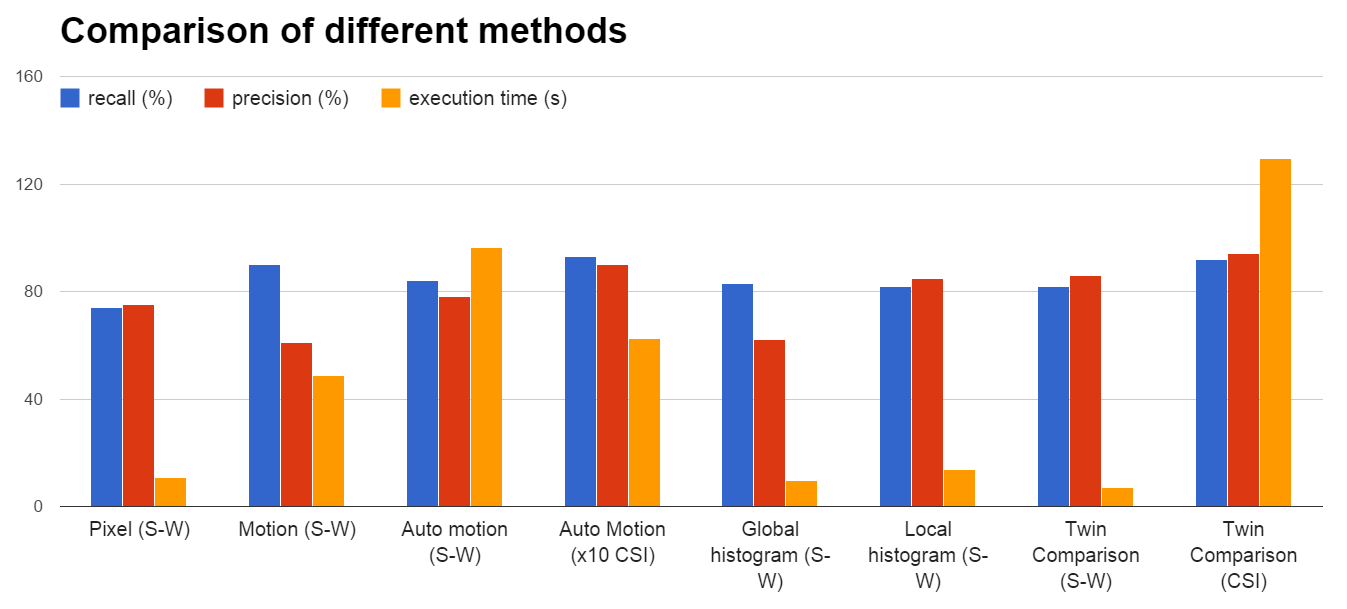
\includegraphics[page=1,angle=90,height=0.74\textheight,keepaspectratio]{grafiek}
  \caption{A comparison of the result}
  \label{grafiek}
\end{figure}

\end{appendices}

\end{document}